\section{Simulation Analysis}
\label{sec:simulation}

\subsection{Operating Point Analysis}

We start by inputing the given circuit into the simulation software, \emph{ngspice}, by numbering the existing nodes and carefully specifying each components connections as shown in figure \ref{Ngspiceinicial}.
One must add that in order to define $V_d$ one needs to have access to the current going through $R_6$, so we added a voltage source $V_{aux}$, with voltage $0V$, connected to nodes 0 and 4, in series with $R_6$ to take its current, since this is the same for components in series.

\begin{figure}[H]
  \centering
  \includegraphics[width=10cm]{../doc/NGSpice_RC}
  \caption{Considered circuit to input in \emph{ngspice}}
  \label{fig:fignodos}
\end{figure}

After inputing all components into \emph{ngspice}, we then ran the simulation program for time $t<0$, in which voltage source $v_s$ has a constant output $V_s$, as indicated in Eqs. \ref{eq:v_s} and \ref{eq:u}. Because $v_s$ is the only independent source in the circuit, the solution reaches a steady-state regime after capacitor $C$ is charged, thus the results are all constant values.


Table \ref{tab:ngspice_1} shows the simulated results for the circuit
under analysis, namely the currents in all branches and the voltages in all nodes.
\begin{multicols}{2}

\begin{table}[H]
  \centering
  \begin{tabular}{|l|r|}
    \hline
    {\bf Name} & {\bf Value [A or V]} \\ \hline
    \input{../sim/op_tab1}
  \end{tabular}
  \caption{Operating point analysis for $t<0$. A variable preceded by @ is of type {\em current}
    and expressed in Ampere; other variables are of type {\it voltage} and expressed in
    Volt.}
  \label{tab:ngspice_1}
\end{table}

\end{multicols}

\par We can see that the node voltages are essentially the same as the ones we got from \textit{Octave}. One can immediately notice that current values for the voltage sources are approximately symmetrical to the ones presented in the theoretical analysis. This is because we have considered the current in the voltage sources going from the negative terminal to the positive one. On the other hand, \emph{ngspice} considers the current the other way around, i.e., entering the positive terminal. [CHECK IF APPLIES]

\par We then proceed to simulate the circuit at $t=0$, where the voltage source switches from being constant to being sinusoidal. At this instant, source $v_s$ has a null output, as one can infer from Eqs. \ref{eq:v_s} and \ref{eq:u}. As the capacitor $C$ was charged, the capacitor will mantain the voltage at its terminals as it starts its discharge. This way, at $t=0$, one can substitute the capacitor C with a constant voltage source $V_x = V(6)-V(8)$, being $V(i)$ the voltage at node $i$ calculated previously for time $t<0$. Since this is another script, we ideally should've taken the 2 node voltages from the previous script to the second, but since the octave's results were essentially the same, we just used the latter while declaring the components. We then ran the operating point analysis. Table \ref{tab:ngspice_2} shows currents in all branches and voltages in all nodes, at time $t=0$.

\begin{multicols}{2}
\begin{table}[H]
  \centering
  \begin{tabular}{|l|r|}
    \hline
    {\bf Name} & {\bf Value [A or V]} \\ \hline
    \input{../sim/op_tab2}
  \end{tabular}
  \caption{Operating point analysis for $t=0$. A variable preceded by @ is of type {\em current}
    and expressed in Ampere; other variables are of type {\it voltage} and expressed in
    Volt.}
  \label{tab:ngspice_2}
\end{table}
\end{multicols}

\par This proceeding is necessary in order to obtain the voltages at nodes 6 and 8 at $t=0$, so that these can be used as border conditions for times $t>0$. 

\subsection{Transient Analysis}

\par We begin by studying the natural response of the circuit, keeping the source $v_s$ null. The following image represents the evolution of voltage $v(6)$ for the time interval [0,20$ms$].

\begin{figure}[H]
  \centering
  \includegraphics[width= 0.45\textwidth]{../sim/natural.pdf}
  \caption{Transient analysis with $v_s =0$ for t$\in$[$0$,$20ms$].}
  \label{fig:sim_1}
\end{figure}

The voltage at the capacitor terminals drops with an exponencial form, as theoretically expected.

\par Now considering that the source $v_s$ has a sinusoidal output, as reffered in Eqs. \ref{eq:v_s} and \ref{eq:u}, we reproduce the same analysis, also presenting the voltage at node 1.


\begin{figure}[H]
  \centering
  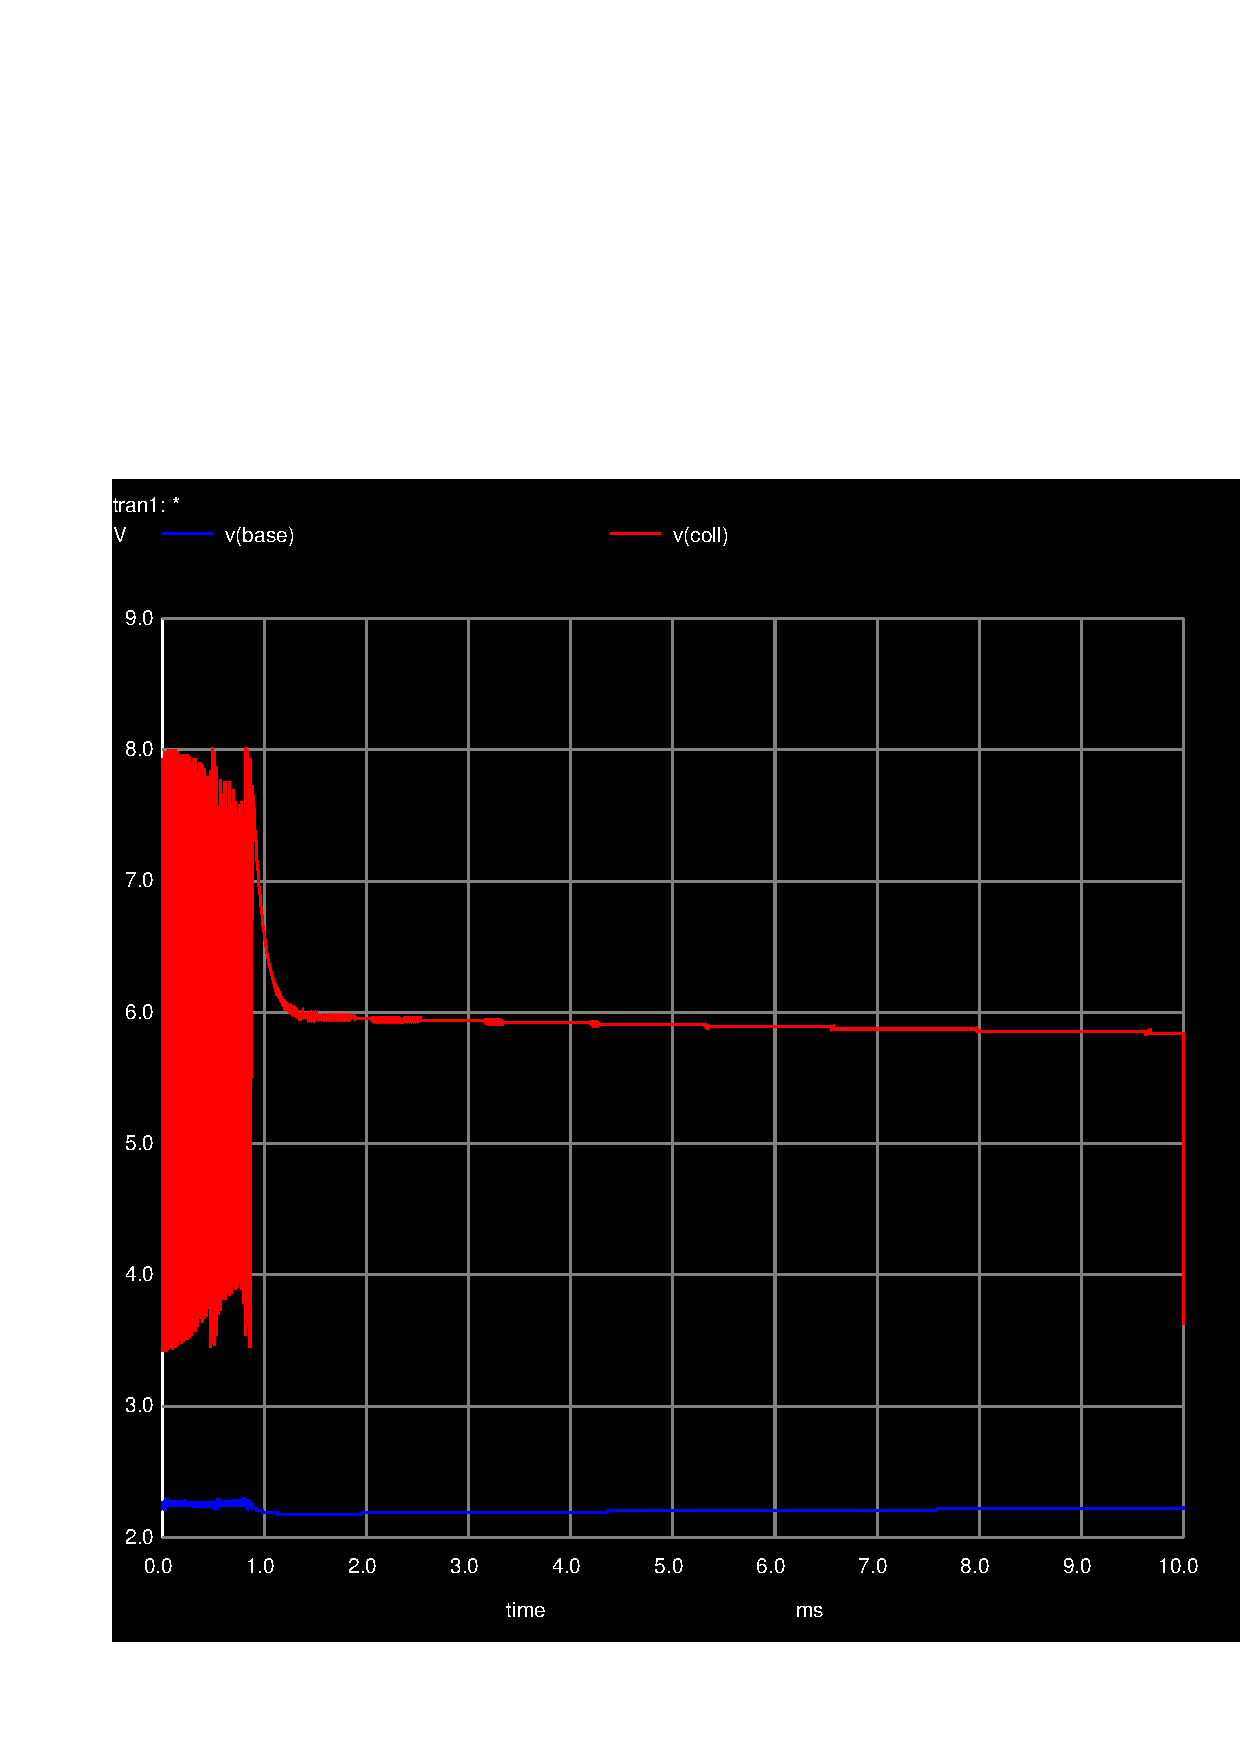
\includegraphics[width= 0.45\textwidth]{../sim/trans.pdf}
  \caption{Transient analysis with $v_s = sin(2\pi 1000 t)$ for t$\in$[$0$,$20ms$].}
  \label{fig:sim_2}
\end{figure}

\par We can see that voltage at node 6 drops as a superposition of the natural and the forced solutions. Beyond time $t=14ms$, the forced response is practically the only in play. The results agree with the theoretical analysis.

\subsection{Frequency Analysis}

\par Next, a frequency analysis was performed, checking the magnitude and phase responses in the range of 0.1$Hz$ to 1$MHz$. The plots are shown bellow.

\begin{figure}[H]
  \centering
  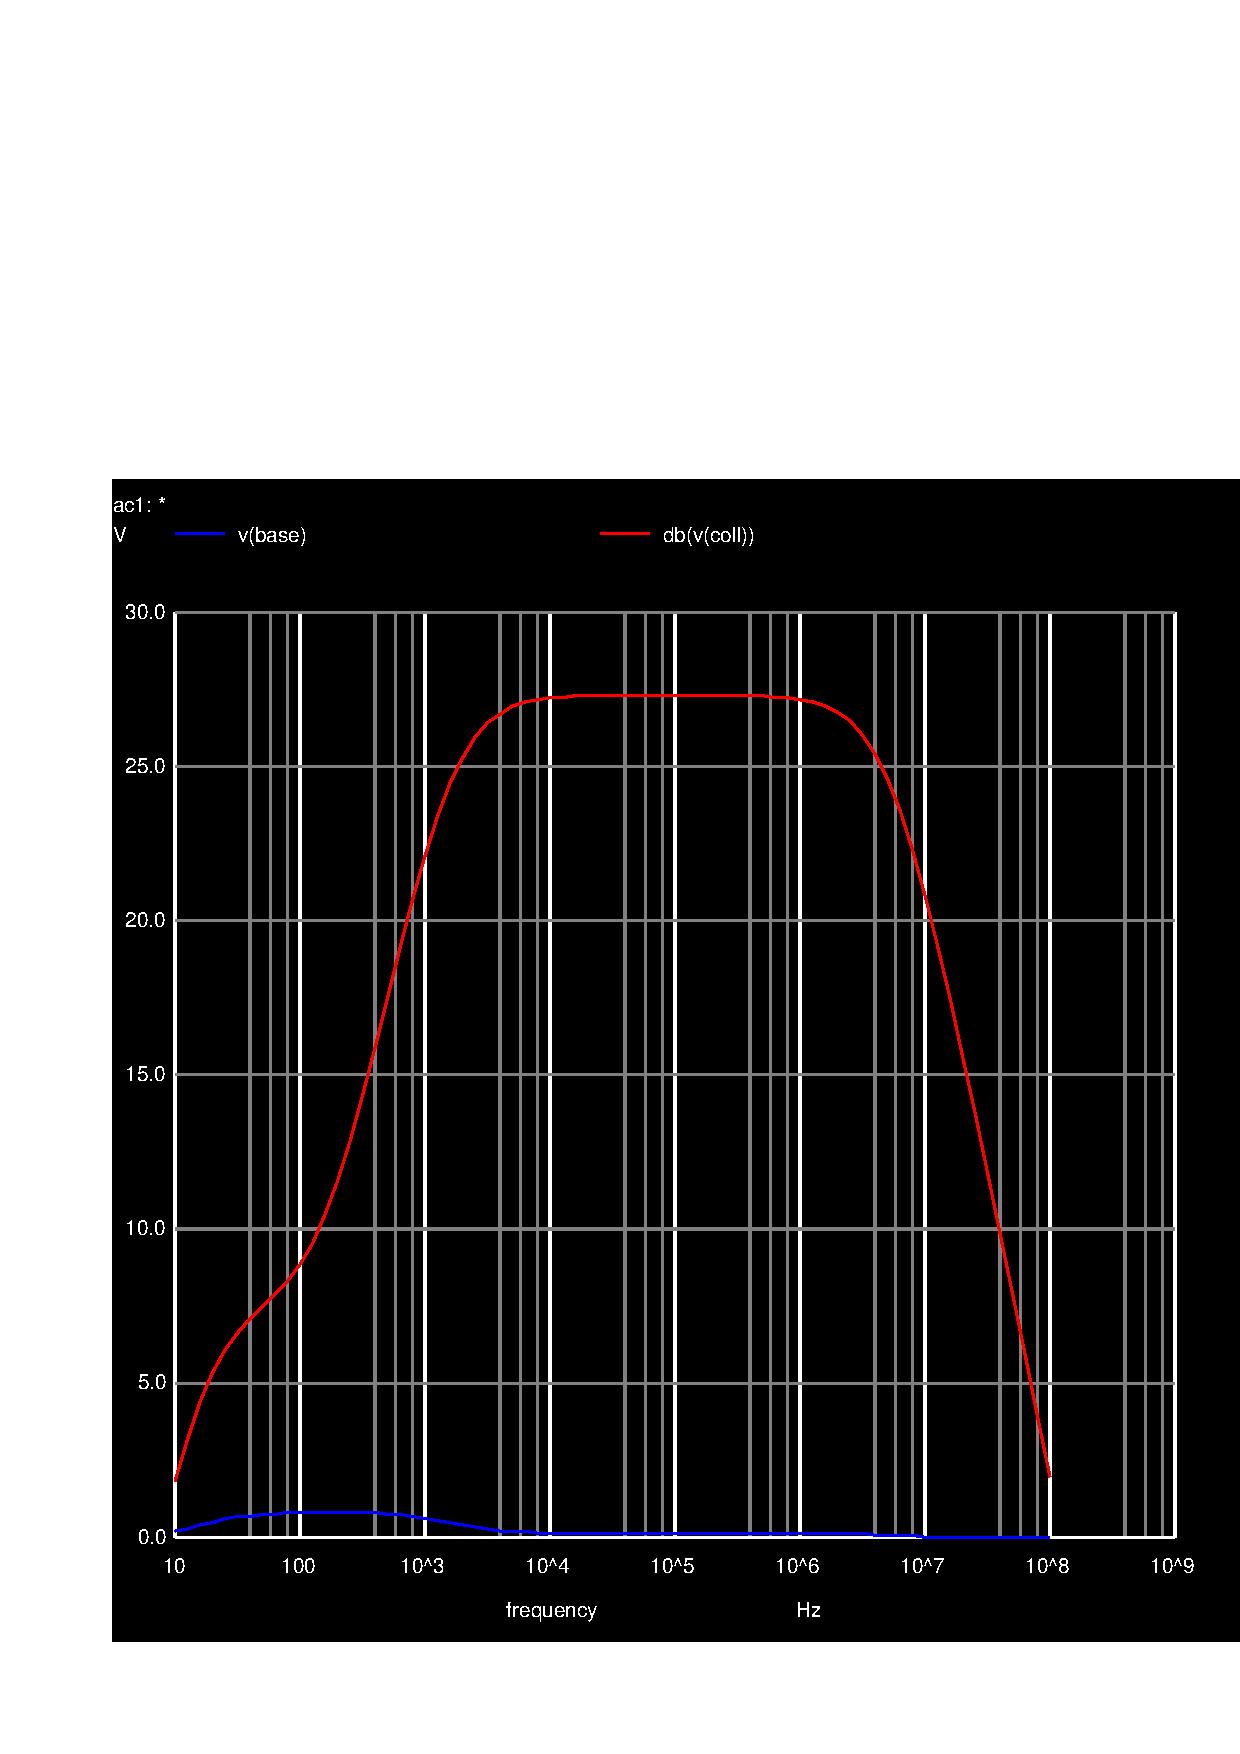
\includegraphics[width= 0.45\textwidth]{../sim/acm.pdf}
  \caption{Frequency analysis. Magnitude in dB. Freq. range in logarathmic scale.}
  \label{fig:sim_3}
\end{figure}

\begin{figure}[H]
  \centering
  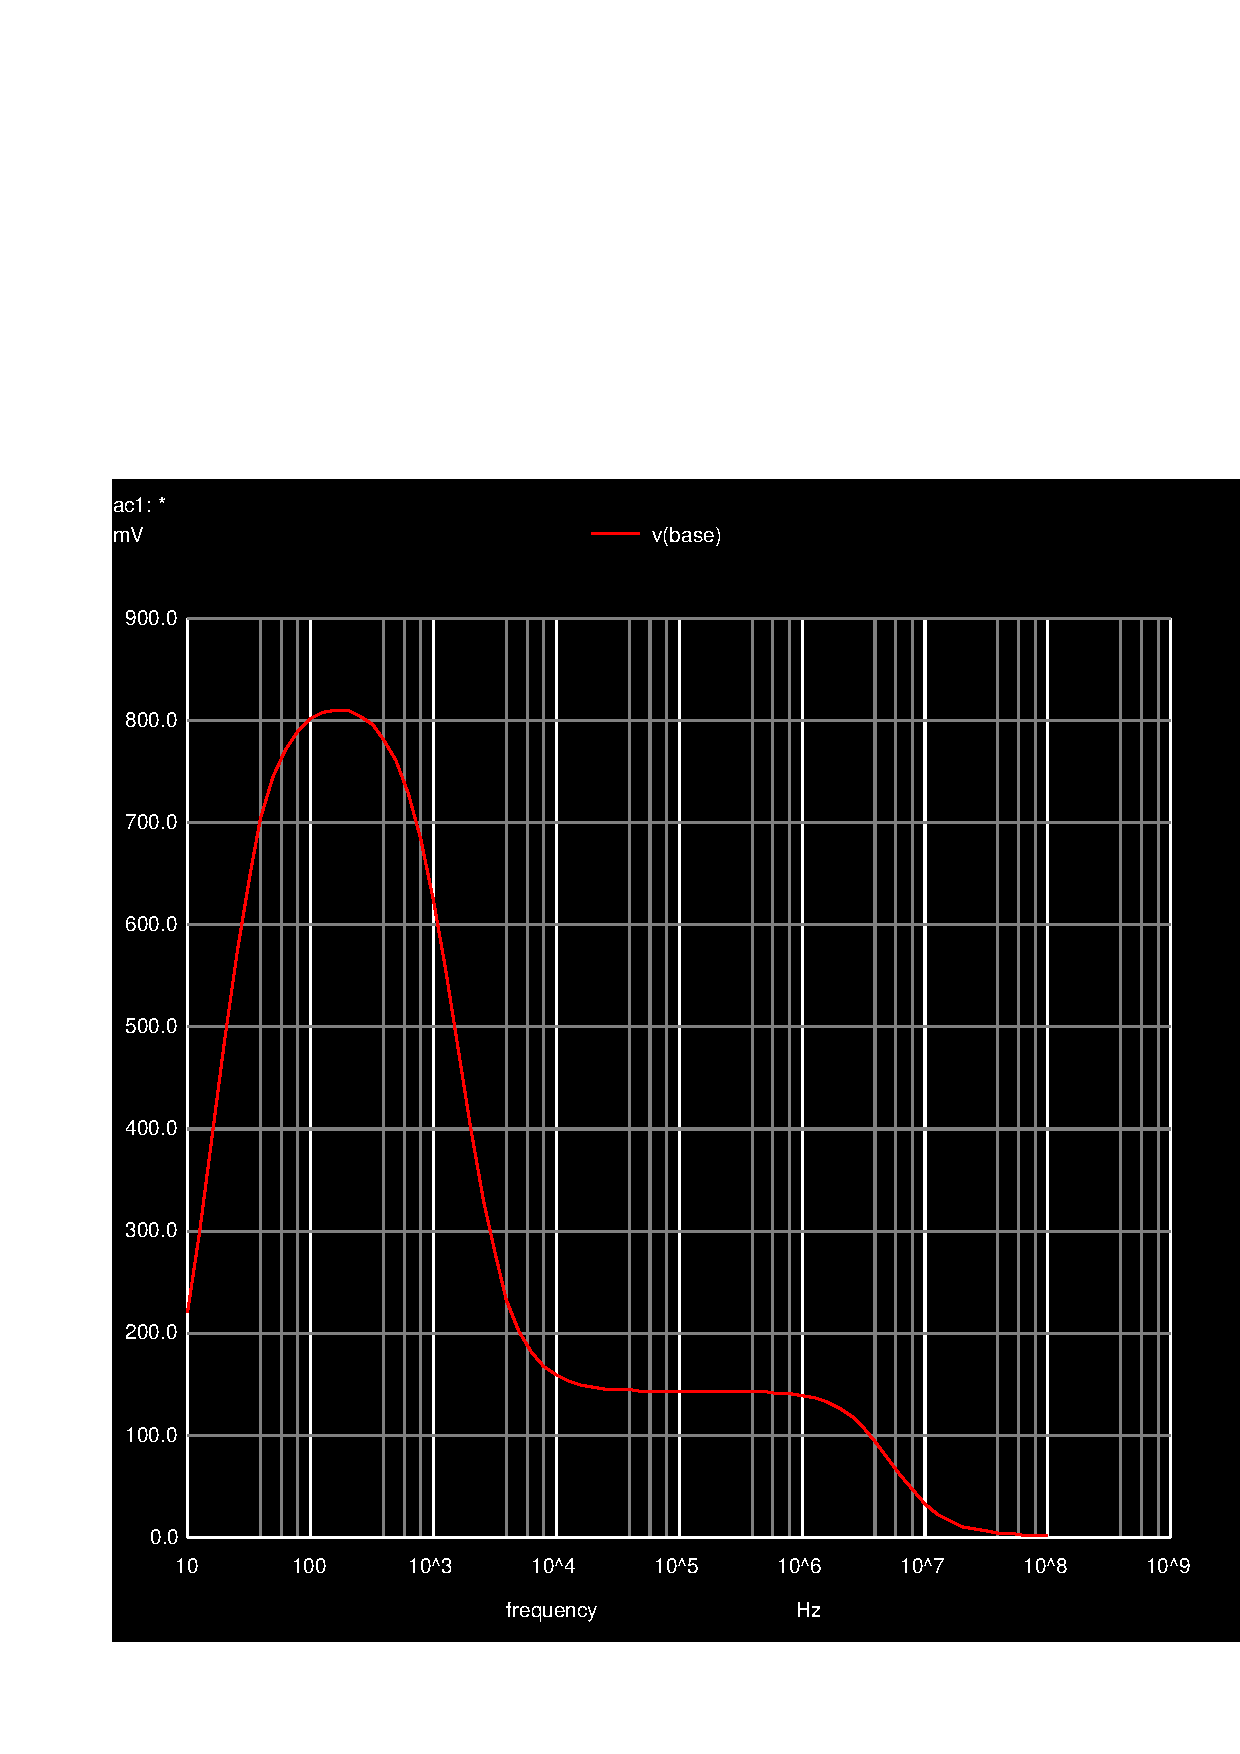
\includegraphics[width= 0.45\textwidth]{../sim/acp.pdf}
  \caption{Frequency analysis. Phase in degrees. Freq. range in logarathmic scale.}
  \label{fig:sim_3}
\end{figure}

\par
We now proceed to calculate the discrepancies between the theoretical analysis and the simulation results:
%formula do erro
\begin{equation}
  \centering
  \epsilon (x_e)=\frac{|x_e-x_r|}{x_r} \times 100\,\%
  \label{eq:error}
\end{equation}

We have considered the value obtained by the mashes/nodes methods as the "real" one ($x_r$) and the value obtained through \emph{ngspice} as the experimental one ($x_e$). It is important to notice, once more, that the values from \emph{ngspice} for the current going through the voltages sources are simetric to the ones we have considered. The percentual error computation had this in mind.

Here, we present the obtained values for the errors.

\begin{table}[H]
  \centering
  \begin{tabular}{|l|r|}
    \hline
    {\bf Name} & {\bf Value in \%} \\ \hline
    %\input{../mat/error_tensoes}
  \end{tabular}
  \caption{Voltages' percentual errors}
  \label{tab:error_tensoes}
\end{table}

Analysing the figure above, the magnitude of $v(1)$, equal to $v_s$ is constant because the magnitude of the imposed voltage is not dependent on the frequency. On the other hand, the impedence of the capacitor follows $Z_c = 1/j\omega C$, thus, according to phasors Ohm's law, the voltage at its terminals tends to zero. 

\begin{table}[H]
  \centering
  \begin{tabular}{|l|r|}
    \hline
    {\bf Name} & {\bf Value in \%} \\ \hline
    %\input{../mat/error_current}
  \end{tabular}
  \caption{Currents' percentual errors }
  \label{tab:error_current}
\end{table}

We have not considered the error in the $8^{th}$ node, since it is defined to be exactly 0. Therefore, the use of equation \ref{eq:error} would give us an infinite answer. However, we have presented the error for $V_a$. Although this voltage was given to us by the \emph{python} code available, \emph{ngspice} is unable to consider the same number of significant figures as the ones presented, resulting in a non-zero value.
